%versi 3 (22-07-2020)
\chapter{Landasan Teori}
\label{chap:teori}

% label: {what for}:{page}:{section}:{subsection}:{name}

\section{SharIF Judge}
\label{sec:2:sharifjudge}

SharIF Judge merupakan modifikasi dari \textit{open source} bernama Sharif Judge, sebuah situs web judge gratis dengan kemampuan mengkompilasi bahasa C, C++, Java, dan Python. Sharif Judge dibuat oleh Mohammad Javad Naderi dengan interface web berbahasa PHP menggunakan \textit{framework} CodeIgniter 3 dan BASH~\cite{javed:sharif}. Modifikasi dilakukan untuk menambahkan fitur pada Sharif Judge dan juga untuk menyesuaikan sesuai dengan kebutuhan Teknik Informatika UNPAR.

\subsection{Instalasi}
\label{sub:2:1:instalasi}

% Ada beberapa prasyarat yang diperlukan dalam menjalankan SharIF Judge pada sebuah \textit{server} Linux adalah sebagai berikut:
Beberapa prasyarat yang diperlukan untuk menjalankan SharIF Judge pada sebuah \textit{server} Linux adalah sebagai berikut:

\begin{itemize}
	\item \textit{Webserver} dengan PHP versi 5.3 atau lebih dengan \texttt{mysqli} extension
	\item PHP Command Line Interface (CLI)
	\item \textit{Database} MySql atau PostgreSql
	\item PHP harus memiliki akses untuk menjalankan \textit{shell commands} dengan fungsi \verb|shell_exec|
	\item Kemampuan untuk mengompilasi dan menjalankan kode yang dikumpulkan (\texttt{gcc}, \texttt{g++}, \texttt{javac}, \texttt{java}, \texttt{python2}, dan \texttt{python3})
	\item Perl
\end{itemize}

% Setelah perangkat yang sudah memenuhi prasyarat, berikut merupakan cara instalasi SharIF Judge:
Setelah perangkat memenuhi prasyarat, berikut merupakan cara instalasi SharIF Judge:

\begin{enumerate}
	\item Unduh versi terakhir dari Sharif Judge dan menempatkannya pada direktori publik.
	\item Pindahkan folder \texttt{system} dan \texttt{application} ke luar direktori publik. Kemudian simpan alamatnya pada \texttt{index.php}.
	\item Buat sebuah \textit{Database} MySql atau PostgreSql.
	\item Atur pengaturan koneksi \textit{database} pada \texttt{application/config/database.php}.
	\item Atur pengaturan \texttt{RADIUS} dan \texttt{SMTP} pada \texttt{application/config/secrets.php} jika dibutuhkan.
	\item Atur agar direktori \texttt{application/cache/Twig} dapat ditulis oleh php.
	\item Buka halaman utama SharIF Judge pada \textit{browser} dan ikuti proses instalasi.
	\item Log in dengan akun admin
	\item Pindahkan folder \texttt{tester} dan \texttt{assignments} ke luar direktori publik. Kemudian simpan alamatnya pada halaman pengaturan.
\end{enumerate}

\newpage

\subsection{Users}
\label{sub:2:1:users}

Pada SharIF Judge, pengguna dibagi menjadi 4 \textit{role}. Role yang tersedia adalah sebagai berikut:

\begin{enumerate}
	\item \textit{admin}
	\item \textit{head instructor}
	\item \textit{instructor}
	\item \textit{student}
\end{enumerate}

Setiap \textit{role} memiliki akses pada aksi yang berbeda berdasakan \textit{role}-nya. Tabel \ref{tab:2:1:fitur_user} merupakan aksi-aksi yang dapat dilakukan untuk setiap pengguna pada SharIF Judge.

\begin{table}[H]
	\centering
	\caption{\textit{Tabel fitur untuk setiap role}}
	\label{tab:2:1:fitur_user}
	\begin{tabular}{|l|c|c|c|c|}
		\hline
		Aksi                              & \textit{Admin} & \textit{Head Instructor} & \textit{Instructor} & \textit{Student} \\

		\hline
		Mengubah \textit{Settings}        & \ding{51}      & \ding{53}                & \ding{53}           & \ding{53}        \\
		Mengelola Pengguna                & \ding{51}      & \ding{53}                & \ding{53}           & \ding{53}        \\
		Mengelola \textit{Assignment}     & \ding{51}      & \ding{51}                & \ding{53}           & \ding{53}        \\

		Mengelola Notifikasi              & \ding{51}      & \ding{51}                & \ding{53}           & \ding{53}        \\
		\textit{Rejudge}                  & \ding{51}      & \ding{51}                & \ding{53}           & \ding{53}        \\
		Mengelola \textit{Queue}          & \ding{51}      & \ding{51}                & \ding{53}           & \ding{53}        \\
		Mendeteksi Kode yang Mirip        & \ding{51}      & \ding{51}                & \ding{53}           & \ding{53}        \\
		Melihat Semua \textit{Submission} & \ding{51}      & \ding{51}                & \ding{51}           & \ding{53}        \\

		Mengunduh Kode Final              & \ding{51}      & \ding{51}                & \ding{51}           & \ding{53}        \\
		Memilih \textit{Assignment}       & \ding{51}      & \ding{51}                & \ding{51}           & \ding{51}        \\
		\textit{Submit} Kode              & \ding{51}      & \ding{51}                & \ding{51}           & \ding{51}        \\

		\hline
	\end{tabular}
\end{table}

\section{CodeIgniter 3}
\label{sec:2:codeigniter}

CodeIgniter 3 adalah sebuah \textit{framework opensource} untuk mempermudah pengguna dalam membangun sebuah aplikasi \textit{website} menggunakan bahasa PHP. CodeIgniter 3 bertujuan untuk membantu pengguna dalam membangun sebuah aplikasi \textit{website} lebih cepat dengan menyedikan \textit{library} yang beragam dengan fungsi yang umum digunakan dan tampilan dan \textit{logic} yang simpel. Gambar \ref{fig:2:ciflowchart} merupakan bagaimana data mengalir pada sistem CodeIgniter.

\begin{figure}[H]
	\centering
	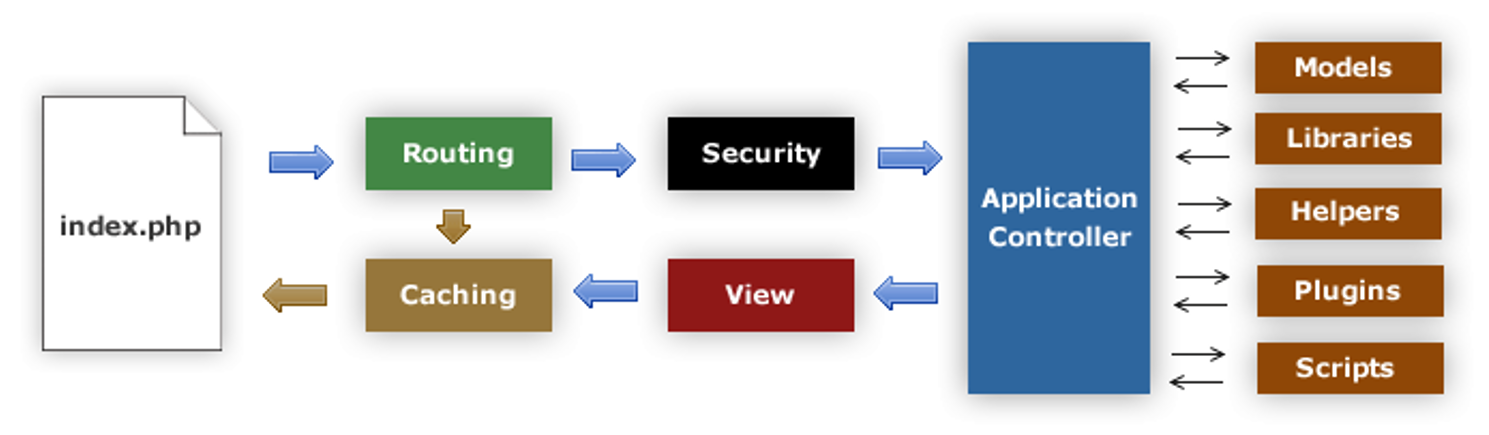
\includegraphics[scale=0.3]{ci-flowchart.png}
	\caption{\textit{Flow Chart} CodeIgniter}
	\label{fig:2:ciflowchart}
\end{figure}

Berikut merupakan penjelasan sederhana dari \textit{flow chart} sistem CodeIgniter 3:

\begin{enumerate}
	\item \verb|index.php| berfungsi sebagai \textit{front controller} yang akan melakukan inisiasi \textit{resource} utama untuk menjalankan CodeIgniter.
	\item Router memeriksa \textit{request} HTTP dan menentukan tindakan selanjutnya sesuai \textit{request} tersebut.
	\item Jika tersedia, \textit{cache} akan langsung dikirimkan ke \textit{browser} melewati proses eksekusi biasa.
	\item Sebelum \textit{controller} dimuat, seluruh \textit{request} HTTP dan data dari pengguna akan disaring terlebih dahulu untuk keamanan sistem.
	\item \textit{Controller} memuat \textit{model}, \textit{library} utama, dan \textit{resource} lainnya yang diperlukan.
	\item \textit{View} akhir lalu dikirim ke browser untuk dilihat.
\end{enumerate}

\subsection{Model-View-Controller}
\label{sub:2:2:modelviewcontroller}

CodeIgniter merupakan framework berbasis arsitektur Model-View-Controller atau yang selanjutnya akan disebut dengan MVC. MVC adalah pendekatan \textit{software} yang memisahkan \textit{logic} aplikasi dan tampilannya. Pendekatan ini membuat \textit{website} hanya memiliki sedikit \textit{script} karena tampilan \textit{website} terpisah dari \textit{scripting} PHP. Berikut merupakan penjelasan mengenai struktur MVC:

\subsubsection{Model}
\label{sub:2:2:1:model}

\textit{Model} mewakili struktur data pada sistem untuk mengambil, memasukkan, dan memperbaharui data pada \textit{database}. \textit{Model} dapat dibuat dengan membuat sebuah kelas yang mewarisi \verb|CI_Model| dan diletakkan pada \verb|application/models/|.

\begin{lstlisting}[language=php, caption=Contoh \textit{model}, label=kode:2:2:1:model]
class Blog_model extends CI_Model {

	public $title;
	public $content;
	public $date;

	public function get_last_ten_entries()
	{
			$query = $this->db->get('entries', 10);
			return $query->result();
	}

	public function insert_entry()
	{
			$this->title    = $_POST['title'];
			$this->content  = $_POST['content'];
			$this->date     = time();

			$this->db->insert('entries', $this);
	}

	public function update_entry()
	{
			$this->title    = $_POST['title'];
			$this->content  = $_POST['content'];
			$this->date     = time();

			$this->db->update('entries', $this, array('id' => $_POST['id']));
	}

}
\end{lstlisting}

Kode \ref{kode:2:2:1:model} merupakan contoh model kelas bernama \verb|Blog_model| pada CodeIgniter. \textit{Model} \verb|Blog_model| dapat mengambil, menambahkan, dan memperbaharui \textit{database} bernama `entries'. File \textit{model} tersebut akan disimpan pada \verb|application/models/Blog_model|. Selanjutnya, pengguna dapat memanggil \textit{Model} tersebut pada \textit{file controller} (akan dijelaskan pada bagian \hyperref[sub:2:2:3:Controller]{Controller}) untuk memuat model pada Kode \ref{kode:2:2:1:model} dengan mengunakan notasi sebagai berikut:

\begin{center}
	\verb|$this->load->model('Blog_model');|.
\end{center}

Untuk memanggil fungsi pada model tersebut, notasi yang digunakan adalah sebagai berikut:

\begin{center}
	\verb|$this->Blog_model->get_last_ten_entries();|
\end{center}

Notasi di atas akan memuat model dengan nama \verb|Blog_model| dan akan memanggil fungsi bernama \verb|get_last_ten_entries|. Notasi untuk memanggil sebuah fungsi dalam model hanya dapat dilakukan jika notasi untuk memuat sebuah model sudah dilakukan sebelumnya.

\subsubsection{View}
\label{sub:2:2:2:View}

\textit{View} adalah informasi yang akan di tunjukkan kepada user. Biasanya \textit{view} merupakan sebuah halaman web, tetapi pada CodeIgniter, view dapat berupa pecahan halaman seperti \textit{header, footer, sidebar}, dan lainnya. Pecahan halaman tersebut dapat dimasukkan secara fleksibel \mbox{ke dalam \textit{view} lainnya apabila dibutuhkan.}

\begin{lstlisting}[language=php, caption={Contoh \textit{view}}, label={kode:2:2:2:view}]
<html>
<head>
        <title>My Blog</title>
</head>
<body>
        <h1>Welcome to my Blog!</h1>
</body>
</html>
\end{lstlisting}

Kode \ref{kode:2:2:2:view} merupakan contoh dari \textit{file view} pada CodeIgniter. File akan disimpan pada direktori \verb|application/views/|. Untuk dapat diperlihatkan dibutuhkannya penggalian halaman pada \mbox{\textit{file controller} dengan cara sebagai berikut:}

\begin{center}
	\verb|$this->load->view(`name');|
\end{center}

Notasi di atas akan mengembalikan halaman \textit{view} dengan nama \verb|name| yang terletak pada direktori \verb|application/views/name.php| dan menampilkannya kepada pengguna.

\subsubsection{Controller}
\label{sub:2:2:3:Controller}

\textit{Controller} adalah bagian utama dari aplikasi CodeIgniter, berfungsi sebagai perantara antara \textit{model}, \textit{view}, dan \textit{resources} lainnya yang dibutuhkan untuk memproses HTTP \textit{request} dan membuat sebuah halaman web. Kelas \textit{Controller} akan mewarisi \verb|CI_Controller| dan disimpan pada \verb|application/controllers/|. Contoh \textit{controller} ditunjukkan pada Kode \ref{kode:2:2:3:controller}.

\begin{lstlisting}[language=php, caption={Contoh \textit{controller}}, label={kode:2:2:3:controller}]
<?php
class Blog extends CI_Controller {

		public function index()
		{
				echo 'Hello World!';
		}

		public function comments()
		{
				echo 'Look at this!';
		}
}
\end{lstlisting}

Kode \ref{kode:2:2:3:controller} berfungsi dalam mengembalikan string sesuai dengan fungsi \textit{controller} yang dipanggil. Nama file \textit{controller} pada direktori \verb|application/controllers/blog.php| dan metode di atas akan dijadikan segmen pada URL seperti berikut:

\begin{center}
	\verb|example.com/index.php/blog/index/|
\end{center}

URL di atas akan mengembalikan sebuah teks `Hello World!'.

\begin{lstlisting}[language=php, caption=Contoh memuat \textit{model} dan menampilkan \textit{view}, label=kode:2:2:3:cimodelview]
class Blog_controller extends CI_Controller {
		public function blog()
		{
				$this->load->model('blog');

				$data['query'] = $this->blog->get_last_ten_entries();

				$this->load->view('blog', $data);
		}
}
\end{lstlisting}

Pada CodeIgniter, \textit{model} dan \textit{view} hanya dapat dimuat melalui controller. Seperti contoh, Kode \ref{kode:2:2:3:cimodelview} akan memuat \textit{model} \verb|blog| dan mengambil data dari \textit{database} melalui model \verb|blog|, lalu menampilkan \textit{view} bernama \verb|blog| yang memuat data tersebut.

\subsection{CodeIgniter URLs}
\label{sub:2:2:codeigniterurls}

URL pada CodeIgniter menggunakan \textit{segment-based approach} dibandingkan dengan \textit{query string approach} yang biasanya dipakai. \textit{Segment-based approach} dirancang untuk \textit{search-engine} dan dapat mempermudah pengguna juga. Berikut merupakan contoh dari URL CodeIgniter:

\begin{center}
	\verb|example.com/news/article/my_article|
\end{center}

Struktur URL pada CodeIgniter juga mengikuti pendekatan MVC (Referensi \ref{sub:2:2:modelviewcontroller}) dan biasanya memiliki struktur pemanggilan fungsi pada controller sebagai berikut:

\begin{center}
	\verb|example.com/class/function/params|
\end{center}

\begin{enumerate}
	\item Segmen pertama mewakili kelas \textit{controller} yang ingin dipanggil.
	\item Segmen berikutnya mewakili fungsi kelas atau \textit{method} yang ingin di panggil.
	\item Segmen ketiga dan selanjutnya mewakili \textit{identifier} atau pengenal dan variable-variable lain yang akan di kirimkan ke \textit{controller}.
\end{enumerate}

\subsection{\textit{Helpers}}
\label{sub:2:2:helpers}

\textit{Helpers} merupakan sebuah kumpulan fungsi untuk membantu dalam sebuah kategori tertentu. \textit{File helpers} terdapat pada direktori \verb|system\helpers| atau \verb|application\helpers|. Penggunaan \textit{helpers} dalam \textit{CodeIgniter} adalah dengan memuat file helpers dalam fungsi kelas \textit{Controller} serupa dengan cara pengguna model, yaitu dengan menggunakan notasi seperti berikut ini:

\begin{center}
	\verb|$this->load->helper(`name')|
\end{center}

Setelah \textit{helper} dimuat dalam fungsi, maka kumpulan fungsi dalam \textit{file helper} dapat langsung dipanggil dalam kode setelah notasi memuat \textit{helper} dipanggil.

\section{Twig}
\label{sec:2:twig}

Twig merupakan sebuah \textit{template engine} untuk PHP. Ada beberapa \textit{expression}, \textit{expression}, atau \textit{statement} yang ditemupakan pada template Twig adalah sebagai berikut:
\begin{itemize}
	\item Pewarisan \textit{Template}
	\item Struktur Kontrol (mengunaan kondisional, \textit{looping})
	\item Filter
	\item Variable pada PHP
\end{itemize}

Pada saat template dievaluasi, semua \textit{variable} atau \textit{expression} akan dibuah menjadi value dan \textit{tag} yang mengontrol logika template. Selain itu twig dapat mengembalikan data sesuai yang tertulis pada \textit{file} seperti normal teks dan HTML \textit{tag}.

\begin{lstlisting}[language={php}, caption={Contoh template Twig}, label={kode:2:twig}]


	<ul id="navigation">
	
		<li>
			<a href="{{item.href}}">
				&nbsp;&nbsp;
				{{ item.caption|upper }}
			</a>
		</li>
	
	</ul>

\end{lstlisting}

Kode \ref{kode:2:twig} merupakan contoh sebuah template Twig. Terdapat dua jenis \textit{delimiter}, yaitu \verb|| dan \verb|{{ ... }}|. \textit{Delimiter} \verb|| digunakan untuk menjalankan sebuah \textit{statement} seperti \textit{for-loops}, sedangkan \textit{delimiter} \verb|{{ ... }}| digunakan untuk mengubah sebuah \textit{variable} atau \textit{expression} menjadi sebuah HTML biasa dengan nilai \textit{variable} atau \textit{expression} tersebut.

\section{Integrated Development Environment}
\label{sec:2:ide}

Intergrated Development Environment (IDE) merupakan sebuah aplikasi yang menyediakan berbagai peralatan yang diperlukan untuk membantu pengembangan perangkat lunak. Beberapa peralatan umum yang dimiliki oleh sebuah IDE adalah sebagai berikut:

\begin{itemize}
	\item \textit{Editor} \\
	      Editor teks sebagai tempat untuk mengetik kode, dapat dilengkapi dengan berbagai fitur seperti \textit{syntax highlighting} (menampilkan teks dengan warna yang berbeda untuk meningkatkan keterbacaan kode sesuai dengan bahasa pemrograman yang digunakan) dan \textit{word completion} (menampilkan prediksi kata yang sedang atau akan diketik oleh pengguna).
	\item \textit{Complier} \\
	      Digunakan untuk menterjemahkan kode program yang dibuat pada editor teks ke dalam sebuah program yang dapat dijalankan oleh komputer.
	\item \textit{Execution} \\
	      Menjalankan kode program yang sudah dikompilasi dari \textit{Editor}, dengan input jika dibutuhkan, dan mengembalikan hasilnya kepada pengguna.
\end{itemize}

\section{Ace}
\label{sec:2:ace}

Ace merupakan \textit{library} yang menyediakan sebuah editor kode yang dapat dimasukkan ke dalam sebuah halaman web dan dikembangkan mengunakan bahasa \textit{Javascript}. Ace memiliki kemampuan yang sama seperti editor kode pada umumnya. Berikut merupakan beberapa fitur utama yang dimiliki dan dapat diaktivasikan pada \textit{library} Ace:

\begin{itemize}
	\item \textit{Syntax highlighting} untuk bahasa pemrograman.
	\item Automatic indent dan outdent.
	\item Kemampuan \textit{cut}, \textit{copy}, dan \textit{paste}.
	\item Kemampuan \textit{drag and drop} teks menggunakan mouse.
	\item Banyak \textit{Cursors} dan \textit{selections}
	\item \textit{Line wrapping}
	\item \textit{Code folding}
\end{itemize}

Untuk mengintegrasikan \textit{library} Ace dalam sebuah halaman web, Ace perlu ditanam dalam halaman web. Salah satu cara untuk menanam Ace ke dalam halaman web adalah dengan mem-\textit{build library} atau menngunduh hasil dari \textit{build} folder bernama \textit{src} versi \textit{pre-packaged} yang disediakan oleh Ace. Hasil dari \textit{building library} Ace adalah sebuah folder yang dapat ditaruh dalam direktori lokal. Dalam folder tersebut, terdapat file \textit{javascript} bernama \verb|ace.js| yang dapat dipanggil dalam halaman web untuk menanam \textit{library} Ace dalam halaman web. Cara untuk menanamkan file tersebut sama dengan cara untuk memasukkan file \textit{javascript} yaitu dengan cara seperti berikut:

\begin{center}
	\verb|<script src="/ace-builds/ace.js" type="text/javascript"></script>|
\end{center}

Setelah \textit{library} Ace ditanam untuk mengakses berbagai macam fitur yang disediakan, maka kelas yang disediakan Ace dapat dipanggil. Berikut merupakan beberapa kelas penting yang terdapat pada library Ace adalah sebagai berikut:

\begin{itemize}
	\item \verb|Ace| \\
	      Kelas \verb|Ace| merupakan kelas utama untuk menyiapkan editor kode Ace pada \textit{browser}. Ace memiliki fungsi utama yang penting yaitu fungsi \verb|edit| yang akan membuat sebuah editor dalam halaman web pada element beridentitas argumen yang diberikan saat dipanggil. Fungsi \verb|edit| akan mengembalikan kelas \verb|Editor|.
	\item \verb|Editor| \\
	      Entri utama untuk fungsionalitas library Ace. Editor sendiri merepresentasikan editor kode yang dibuat pada halaman web. Editor juge menjadi kelas utama untuk mengakses kelas-kelas yang berhubungan dengan editor kode dengan mengakses kelas variable \verb|Editor| seperti \verb|session| dalam editor kode. Kelas \verb|Editor| sendiri dapat dikonfigurasikan sesuai dengan fungsi yang disediakan seperti \verb|setTheme| yang mengubah warna editor \mbox{kode sesuai dengan \textit{theme} yang dipilih.}
	\item \verb|EditSession| \\
	      Sebuah kelas yang menyimpan semua status dalam editor seperti isi editor, \textit{selection}, dan lain-lain. Kelas ini dinamakan \verb|EditSession|, tetapi untuk mengakses dari kelas \verb|Editor|, variable \verb|EditSession| dinamakan \textit{session}.
	\item \verb|Anchor| \\
	      Menangani posisi \textit{pointer} pada dokumen. Saat teks dimasukkan atau dihapus, posisi \textit{anchor} akan diperbaharui sesuai dengan teks yang dimasukkan atau dihapus dari dokumen.
	\item \verb|Document| \\
	      Menyimpan teks dokumen.
	\item \verb|Range| \\
	      Kelas ini digunakan di berbagai tempat untuk mengindikasikan suatu wilayah di dalam editor. Kelas ini menyimpan posisi baris awal dan kolom awal, serta baris akhir dan kolom akhir.
	\item \verb|Selection| \\
	      Kelas ini menyimpan posisi yang di pilih oleh pengguna dalam editor.
	\item \verb|Commands| \\
	      Kelas ini digunakan untuk menjalankan perintah pada sebuah editor. Contoh perintah yang sudah ada dalam editor yaitu \textit{insert}, \textit{copy}, \textit{paste}.
\end{itemize}

\begin{lstlisting}[language={html}, caption={Contoh kode pengunaan Ace}, label={kode:2:5:ace}]
<!DOCTYPE html>
<html lang="en">
<head>
<title>ACE in Action</title>
<style type="text/css" media="screen">
	#editor { 
		position: absolute;
		top: 0;
		right: 0;
		bottom: 0;
		left: 0;
	}
</style>
</head>
<body>

<div id="editor">function foo(items) {
	var x = "All this is syntax highlighted";
	return x;
}</div>
	
<script src="/ace-builds/ace.js" type="text/javascript"></script>
<script>
	var editor = ace.edit("editor");
	editor.setTheme("ace/theme/monokai");
	editor.session.setMode("ace/mode/javascript");
</script>
</body>
</html>
\end{lstlisting}

Kode \ref{kode:2:5:ace} merupakan cara pengunaan Ace pada sebuah \texttt{div} dengan id \texttt{editor}. Ace juga memiliki beberapa konfigurasi, seperti contoh ini yaitu mengunakan tema \textit{monokai} dan mengunakan \textit{syntax highlighting} untuk bahasa pemrograman JavaScript. Gambar \ref{fig:2:5:ace} menunjukkan hasil halaman web yang dibuka dalam \textit{browser} menggunakan Kode \ref{kode:2:5:ace}.

\begin{figure}[H]
	\centering
	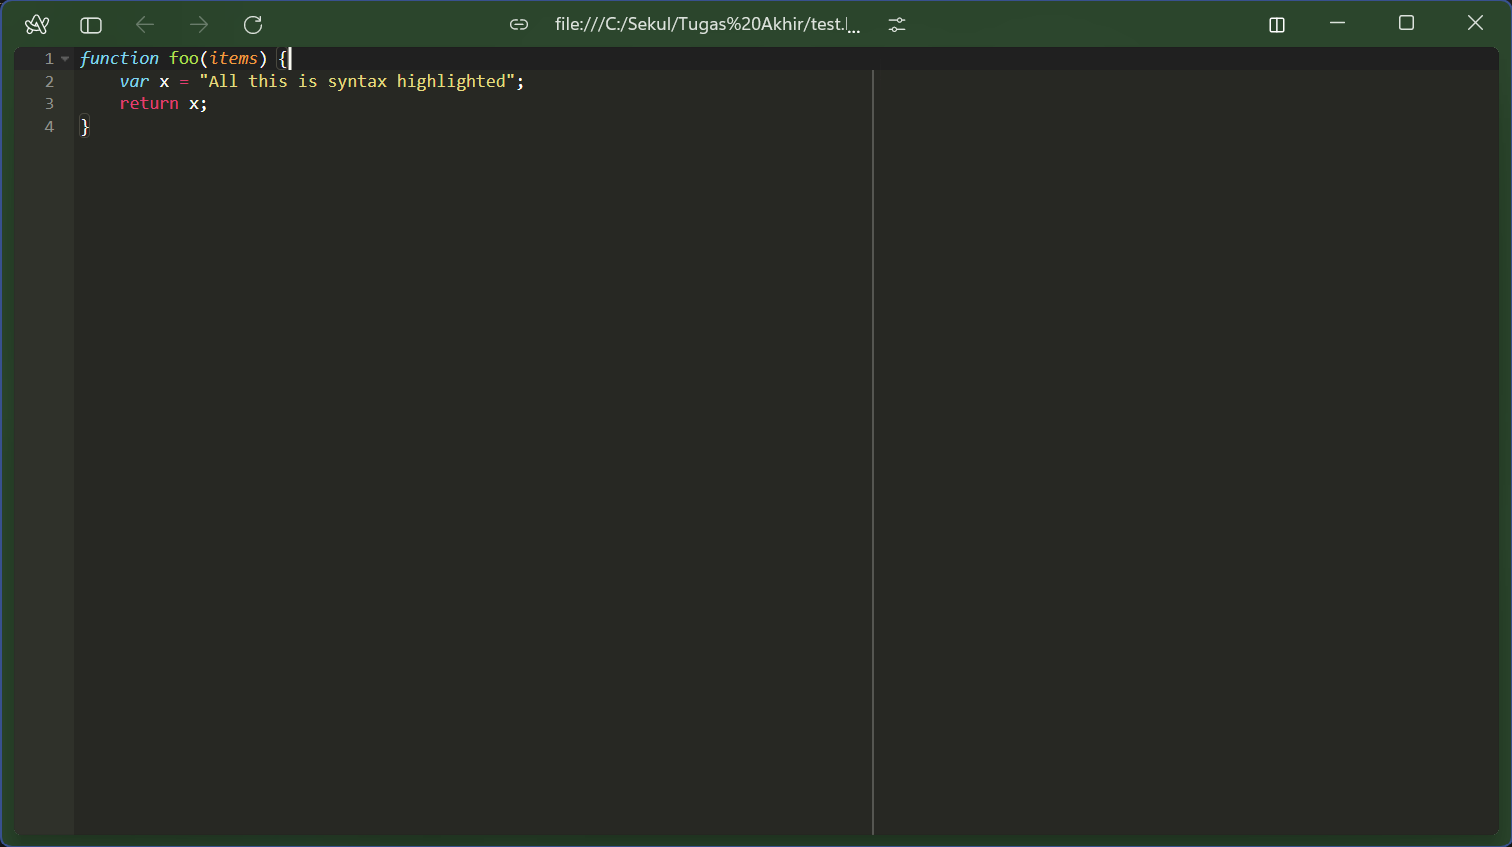
\includegraphics[width=0.65\textwidth]{ace.png}
	\caption{Hasil Halaman Web \textit{Library} Ace}
	\label{fig:2:5:ace}
	\vspace{-1cm}
\end{figure}

\subsection{Perekaman Event}

Pada \textit{library} Ace, disediakannya fungsi \textit{event listener} atau pendengar \textit{event} atau kejadian yang berhubungan dengan kelas-kelas yang disediakan. Pada \textit{event listener} ini akan disediakannya sebuah fungsi \textit{callback} yang akan dipanggil saat \textit{event} tersebut terjadi. Berikut merupakan beberapa \textit{event listener} dalam kelas-kelas yang disediakan oleh \textit{library} Ace:

\begin{itemize}
	\item \verb|Editor| \\
	      Pada editor sendiri disediakannya satu \textit{event listener} yaitu \verb|mouseup| yang akan mendengarkan saat melepaskan tombol pada tetikus atau \textit{mouse}.

	\item \verb|EditSession| \\
	      Pada kelas \textit{session} ada satu \textit{event listener} yaitu \verb|change| yang akan mendengarkan perubahan pada isi atau kode pada editor kode. Pada fungsi \textit{callback} yang akan dijalankan oleh \textit{event listener} ini akan diberikan objek \textit{javascript} bernama \verb|delta| yang menunjukkan perubahan dan lokasi terjadi perubahan pada editor kode.

	\item \verb|Selection| \\
	      Pada kelas \textit{selection} ada beberapa \textit{event listener} yaitu sebagai berikut:

	      \begin{itemize}
		      \item \verb|changeCursor| : Mendengarkan perubahan pada kursor atau \textit{anchor} dalam editor kode.
		      \item \verb|changeSelection| : Mendengarkan perubahan pemilihan isi kode dalam editor kode.
	      \end{itemize}

	\item \verb|Commands| \\
	      Pada kelas ini tersedia dua \textit{event listener} yaitu \verb|exec| dan \verb|afterExec|. \verb|exec| akan mendengarkan saat perintah akan dijalankan pada editor kode, sedangkan \verb|afterExec| akan mendengarkan perintah yang sudah selesai dijalankan pada editor kode. Pada fungsi \textit{callback} yang akan dijalankan oleh \textit{event listener} ini akan diberikan perintah yang dijalankan oleh kelas \verb|Commands|.
\end{itemize}

Untuk menggunakan fungsi \textit{event listener} pada kelas yang diinginkan, dibutuhkan fungsi \verb|on| pada kelas tersebut. Fungsi \verb|on| memiliki dua parameter yaitu nama \textit{event} yang ingin didengar (\verb|exec| atau \verb|change|) dan sebuah fungsi \textit{callback} yang akan dijalankan saat \textit{event} terjadi. Kode \ref{kode:2:5:1:eventlistener} merupakan perubahan kode yang dilakukan dalam \textit{tag} \verb|<script>| pada Kode \ref{kode:2:5:ace} agar perubahan isi editor dapat didengar dan akan mengeluarkan perubahan yang dilakukan pada editor kode.

\begin{lstlisting}[language={html}, caption={Contoh kode event listener}, label={kode:2:5:1:eventlistener}]
<script src="/ace-builds/ace.js" type="text/javascript"></script>
<script>
	var editor = ace.edit("editor");
	editor.setTheme("ace/theme/monokai");
	editor.session.setMode("ace/mode/javascript");

	editor.session.on("change", (delta) => {
        console.log(delta);
		// Contoh Keluaran :
		// {
		// 		action: "insert"
		// 		end: {row: 3, column: 5}
		// 		lines: ['a']
		// 		start: {row: 3, column: 4}
		// }
	});
</script>
\end{lstlisting}

Kode \ref{kode:2:5:1:eventlistener} akan menggunakan \textit{event listener} \verb|change| dalam kelas \verb|EditSession|, dengan mengakses kelas \verb|EditSession| melalui \verb|editor| yang dinamakan \verb|session|. Pada kelas tersebut akan dijalankan fungsi \verb|on| dengan parameter ``change'' dan sebuah fungsi annonimus sebagai fungsi \textit{callback} yang akan dicetak ke \textit{console} isi perubahan pada editor kode.

\section{Chart.js}

Chart.js merupakan sebuah \textit{library javascript open-source} untuk membuat visualisasi data bagan interaktif berbasis \verb|canvas| dalam halaman web~\cite{chartjs}. Chart.js memiliki fitur-fitur yang dapat digunakan untuk mendukung dan mempermudah visualisasi data dalam halaman web. Berikut merupakan beberapa fitur yang dimiliki oleh Chart.js:

\begin{itemize}
	\item Chart.js menyediakan berbagai tipe bagan yang dapat digunakan dan juga memiliki opsi penyesuaian yang sering digunakan.
	\item Chart.js memiliki konfigusari bawaan yang membuat visualisasi bagan sudah bagus.
	\item Chart.js mudah untuk diintegrasikan dalam sebuah halaman web.
	\item Chart.js mengunakan \textit{canvas HTML5 rendering} yang membuat pembuatan bagan sangat cepat terutama jika data yang dimasukkan sangat besar.
\end{itemize}
 
Identik dengan \textit{library} Ace untuk menintegrasikan \textit{library} Chart.js dalam sebuah halaman web, \textit{library} Chart.js dapat di\textit{build} dan dimasukkan ke dalam folder projek dan menambahkan file \textit{javascript} bernama \verb|chart.js| dalam folder \textit{dist} ke dalam halaman web menggunakan cara yang identik dengan cara memasukkan file \textit{javascript} pada umumnya yaitu dengan cara sebagai berikut:

\begin{center}
	\verb|<script src="/chartjs/dist/chart.js" type="text/javascript"></script>|
\end{center}

Setelah itu \textit{library} Chart.js dapat digunakan dengan membuat sebuah kelas \textit{javascript} baru bernama \verb|Chart|. Untuk membuat kelas \verb|Chart| dibutuhkan 2 argumen yaitu elemen \textit{canvas} dalam HTML halaman web dan sebuah objek \textit{javascript} yang dapat diisi dengan opsi-opsi yang diinginkan dengan menspesifikan \textit{key} dan \textit{value} yang sesuai dengan opsi yang diinginkan. Berikut merupakan beberapa \textit{key} dan \textit{value} yang dapat digunakan ada dalam opsi \textit{library} Chart.js:

\begin{itemize}
	\item \verb|type| \\
	\verb|type| hanya menerima sebuah kata yang menjadi tipe utama bagan yang dibuat oleh \textit{library} Chart.js, tetapi tipe ini dapat berubah mengikuti data yang diberikan. Berikut merupakan beberapa tipe-tipe yang ada dalam \textit{library} Chart.js:
	\begin{itemize}
		\item \verb|bar| \\
		Bagan \verb|bar| menyediakan cara untuk menvisualisasikan data sebagai batang vertikal maupun horizontal. Bagan ini biasanya digunakan untuk menunjukkan data tren dan perbandingan beberapa set data secara berdampingan.
		\item \verb|line| \\
		Bagan \verb|line| adalah cara menvisualisasikan data sebagai titik data yang disambungkan dengan garis. Identik dengan Bagan \verb|bar|, Bagan \verb|line| juga digunakan untuk menunjukkan data tren dan perbandingan beberapa set data secara berdampingan.
	\end{itemize}

	\item \verb|data| \\
	\verb|data| sendiri menerima \textit{value} objek \textit{javascript} dengan isi \verb|labels| dan \verb|dataset|. Kedua \textit{key} menerima sebuah \textit{array} dengan isi yang berbeda. \verb|labels| hanya menerima sebuah \textit{array} berisi teks untuk label data horizontal atau vertikal. \verb|dataset| menerima \textit{array} primitive type, \textit{array} dengan isi \textit{array}, dan \textit{array objek}. \textit{objek} dalam \verb|dataset| menerima \textit{key} \verb|data| dan juga memiliki beberapa \textit{key} opsi yaitu \verb|label| untuk melabelkan data dalam horizontal maupun vertikal. \textit{Key} \verb|data| menerima array dengan isi \textit{array objek} dengan data yang ingin divisualisasikan.

	\item \verb|options| \\
	\textit{Key} \verb|options| merupakan fitur utama dari kelas \verb|Chart| dan hanyak menerima sebuah objek \textit{javascript} yang memiliki banyak \textit{key} untuk menyesuaikan bagan yang dibuat oleh \textit{library} Chart.js. Salah satu \textit{key} dalam \verb|options| adalah \verb|scales| yang digunakan untuk mengatur data yang ditampilakan untuk aksis X dan Y. Salah satu pengaturannya adalah untuk menumpuk data dengan data yang sama di aksis yang sama yaitu dengan mengunakan \textit{key} \verb|stacked|.
\end{itemize}

\begin{lstlisting}[language={html}, caption={Contoh kode pengunaan Chart.js}, label={kode:2:6:chartjs}]
<!DOCTYPE html>
<html lang="en">
<body>
<div>
  <canvas id="myChart"></canvas>
</div>

<script src="https://cdn.jsdelivr.net/npm/chart.js"></script>

<script>
  const ctx = document.getElementById('myChart');

  new Chart(ctx, {
    type: 'bar',
    data: {
      labels: ['Red', 'Blue', 'Yellow', 'Green', 'Purple', 'Orange'],
      datasets: [{
        label: '# of Votes',
        data: [12, 19, 3, 5, 2, 3],
        borderWidth: 1
      }]
    },
    options: {
      scales: {
        y: {
          beginAtZero: true
        }
      }
    }
  });
</script>
</body>
</html>
\end{lstlisting}

Kode \ref{kode:2:6:chartjs} merupakan contoh penggunaan \textit{library} Chart.js pada sebuah \textit{canvas} dengan id \verb|myChart|. \textit{Key} \verb|options| pada contoh ini mengunakan \verb|beginAtZero| yang membuat data dimulai dari nol. Gambar \ref{fig:2:6:chartjs} merupakan hasil halaman web yang dibuka dalam \textit{browser} dengan Kode \ref{kode:2:6:chartjs}.

\begin{figure}[H]
	\centering
	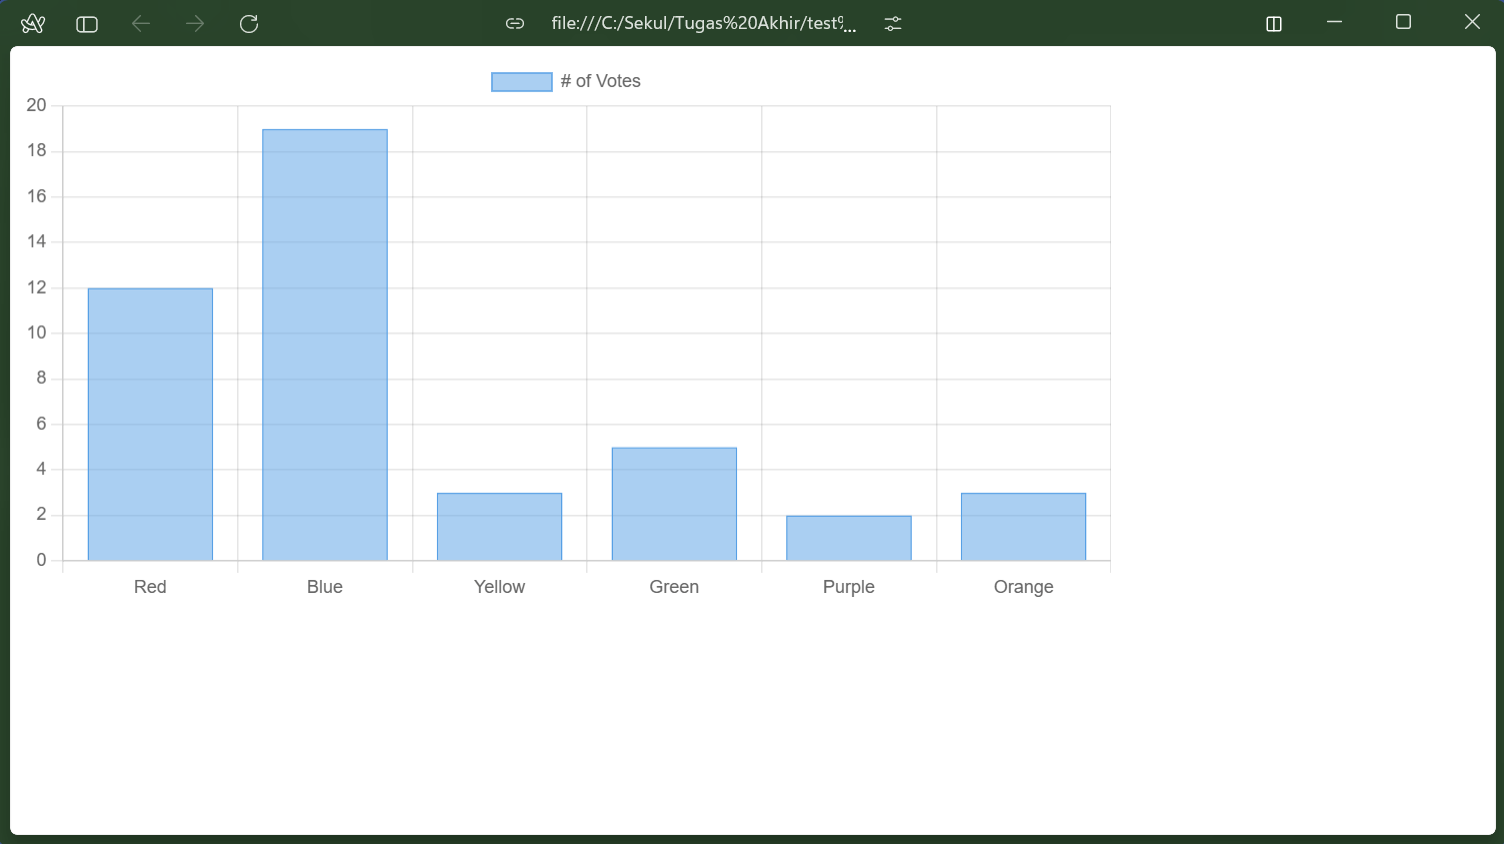
\includegraphics[width=0.7\textwidth]{chartjs.png}
	\caption{Hasil Halaman Web \textit{Library} Chart.js}
	\label{fig:2:6:chartjs}
\end{figure}